\section{Results and Analysis}
% We chose to validate our PoC using a few scenes from Bitterli's 32 resources 
% \cite{resources16}: \textit{The Wooden Staircase} and \textit{Utah Teapot}. 
% These two were chosen for providing a collection of varied directives.

% \textit{The Wooden Staircase} makes use of image-based textures, area lighting 
% and has a vast array of different kinds of materials, including bumpmaps. The 
% scene uses 774 external 3D meshes, which makes manual conversion hard and time consuming, as well as primitive directives, such as rectangles.
% 
% The \textit{Utah Teapot} is a much simpler scene, with two materials, one primitive  and one 
% external 3D mesh. It does, however, use a primitive checkerboard texture and 
% environment mapping.

The scenes were rendered using Mitsuba 0.5.0, PBRT v3 and LuxRender v1.6 on 
%a UNIX system running
Ubuntu 14.04 LTS. All scenes were rendered using over 5,000 samples per pixel. 

% We rendered the original scenes for Mitsuba, PBRT and LuxRender. After that, we 
% rendered the scenes converted from these input files by our system. The original 
% scenes for Mitsuba and PBRT were the ones provided in Bitterli's resources, 
% while the LuxRender scenes were generated using our system.

\begin{figure*}
\centering
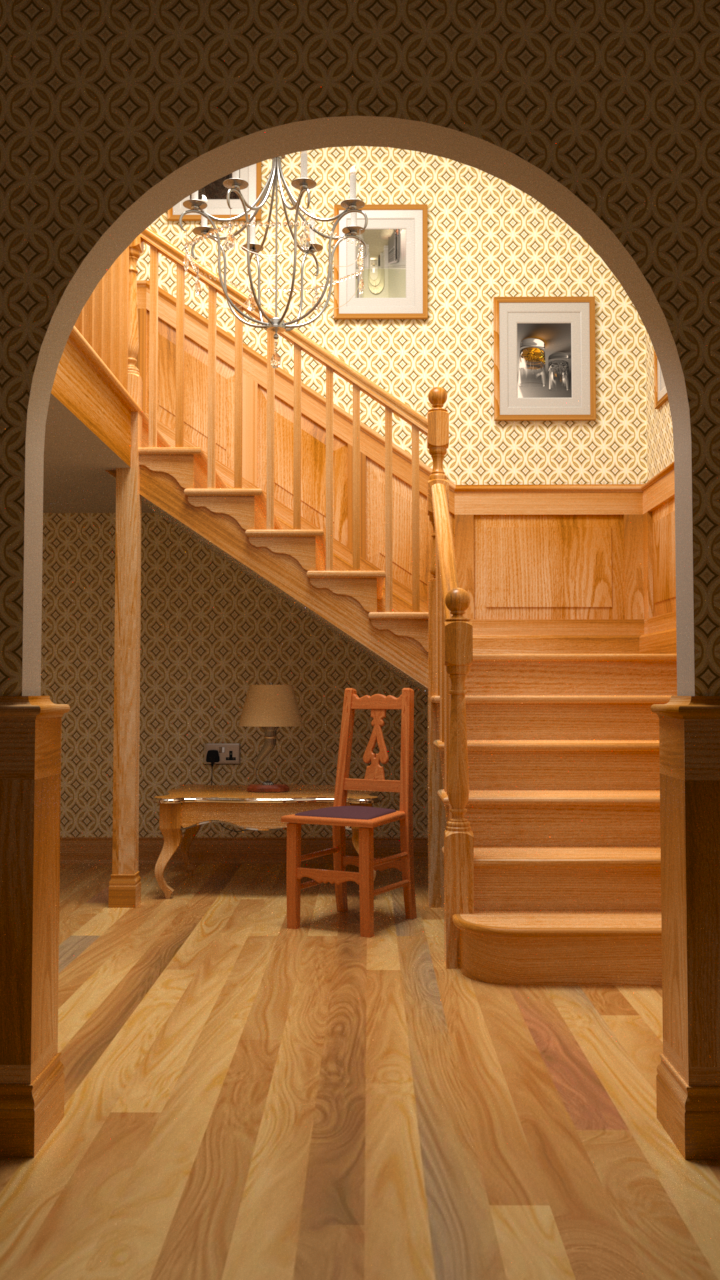
\includegraphics[width=1.5in]{figs/4_results/staircase/1_from_lux.png}
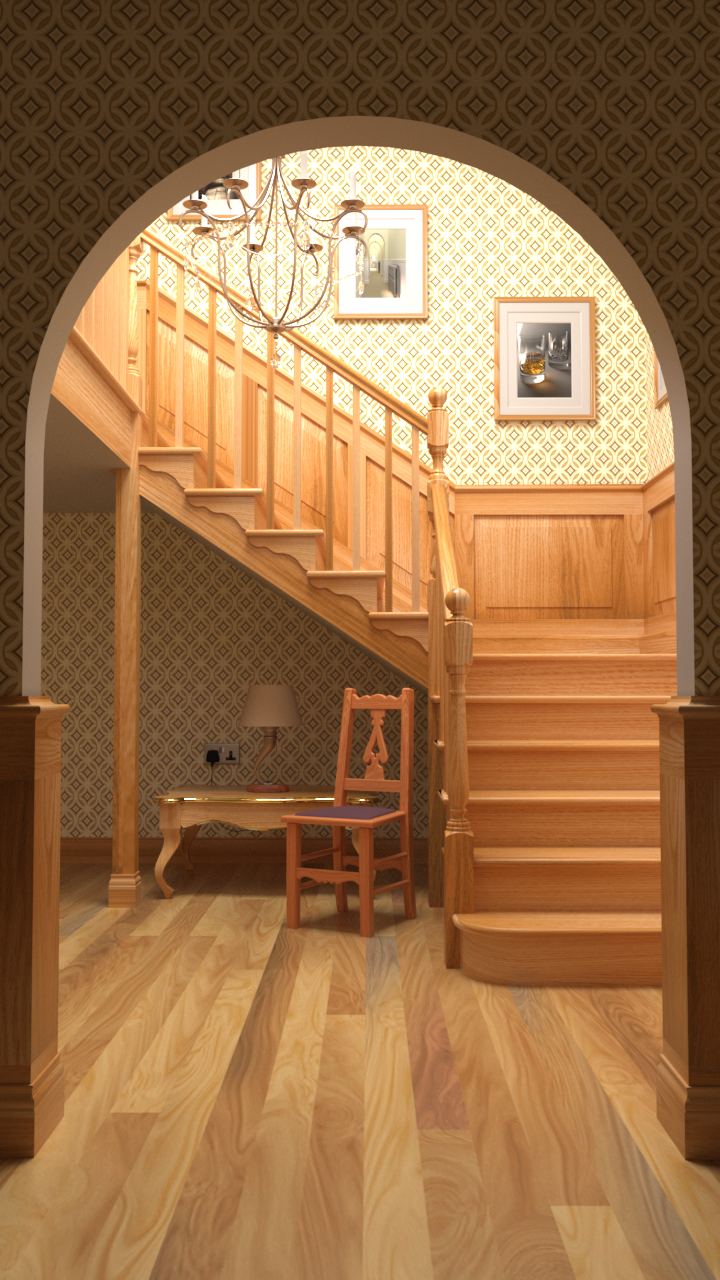
\includegraphics[width=1.5in]{figs/4_results/staircase/2_to_mitsuba.png}
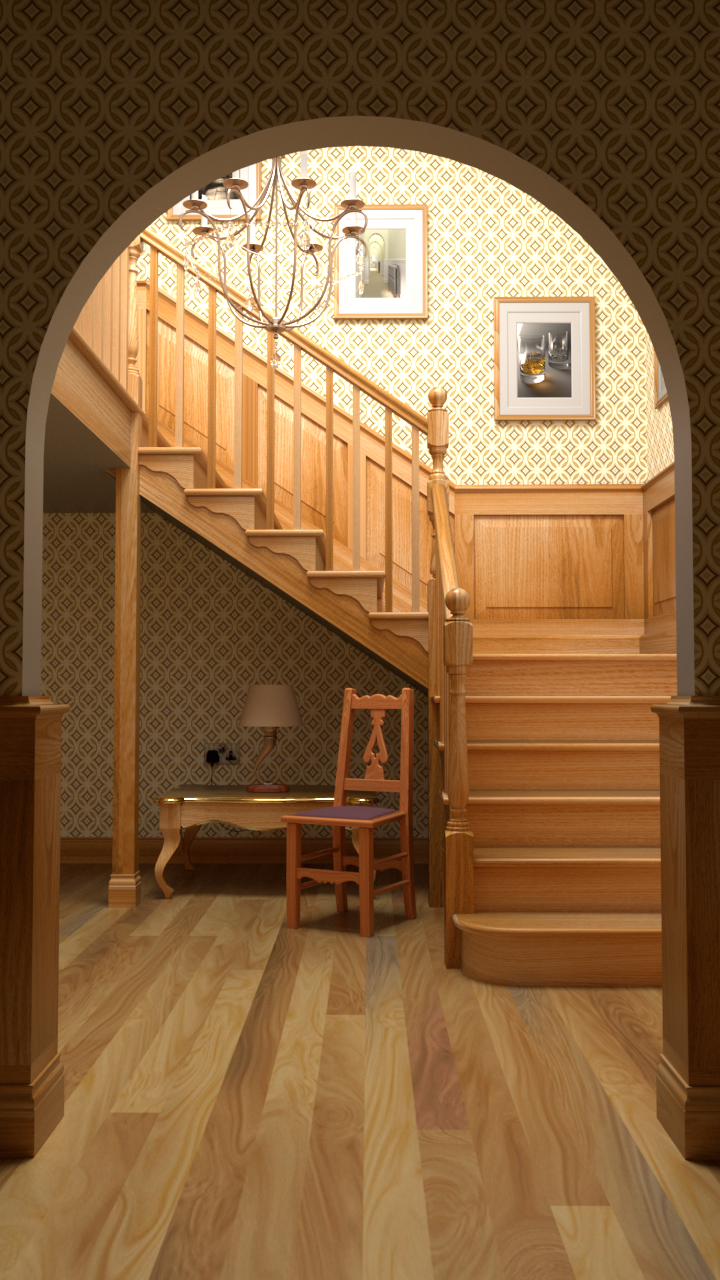
\includegraphics[width=1.5in]{figs/4_results/staircase/3_to_pbrt.png}
\caption{Automatic conversion obtained with our system for \textit{The Wooden Staircase}
scene, originally modeled for LuxRender. Rendering produced by LuxRender (left).
Rendering produced by Mitsuba (center) and PBRT v3 (right),
from converted scenes for the renderers}
\label{fig:staircase}
\end{figure*}

\begin{figure*}
\centering
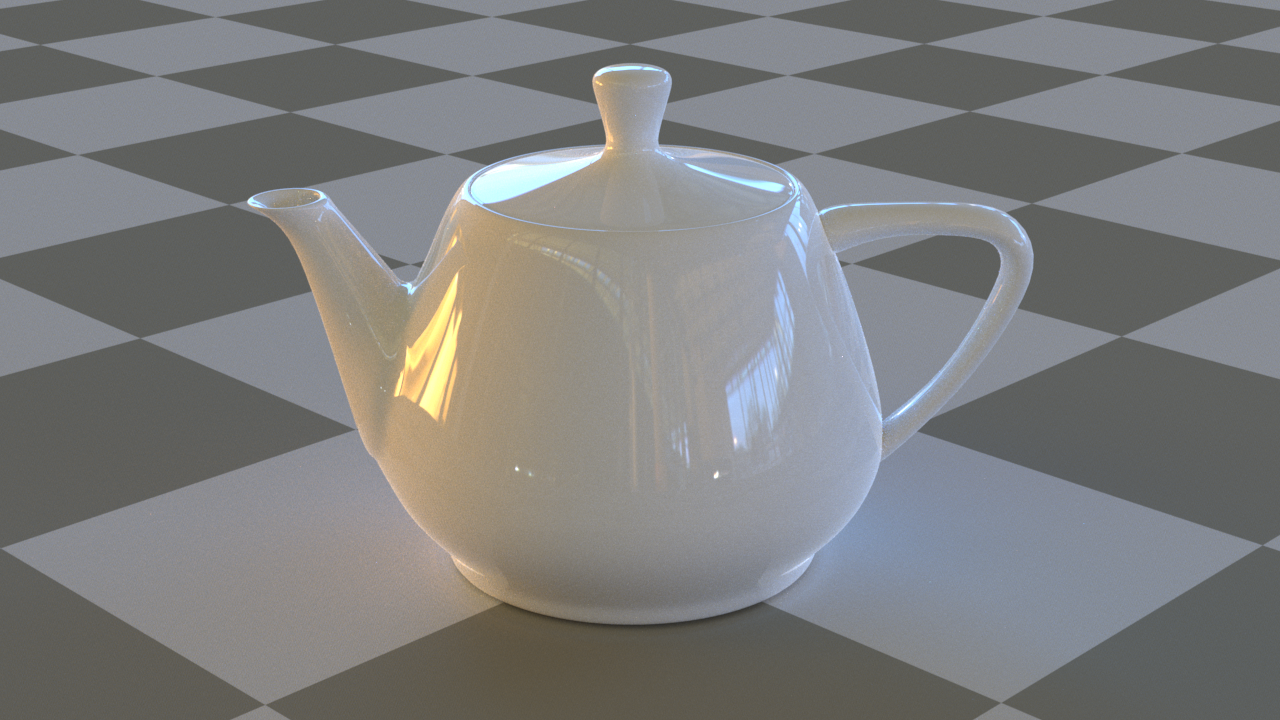
\includegraphics[width=2in]{figs/4_results/teapot/1_from_lux.png}
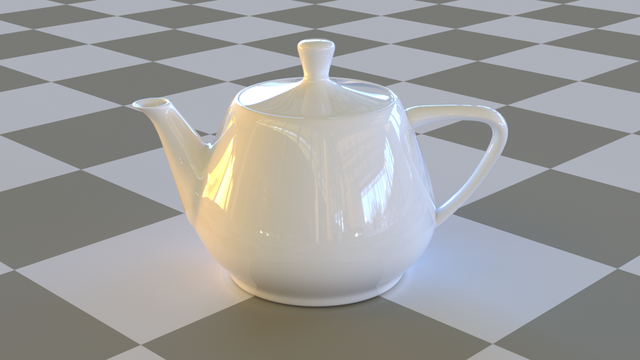
\includegraphics[width=2in]{figs/4_results/teapot/2_to_mitsuba.png}
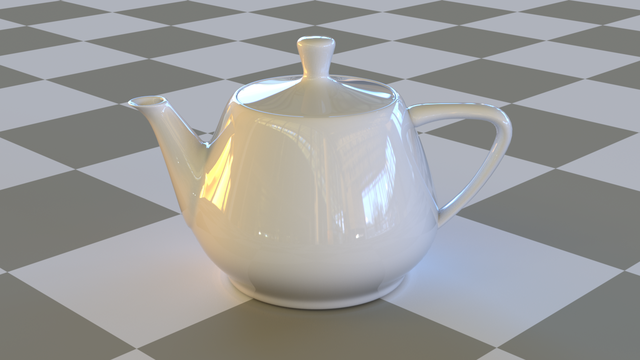
\includegraphics[width=2in]{figs/4_results/teapot/3_to_pbrt.png}
\caption{Automatic conversion obtained with our system for \textit{Utah Teapot}
scene originally modeled for LuxRender. Rendering produced by LuxRender (left).
Rendering produced by Mitsuba (center) and PBRT v3 (right),
from converted scenes for the renderers}
\label{fig:teapot}
\end{figure*}

\begin{figure*}
\centering
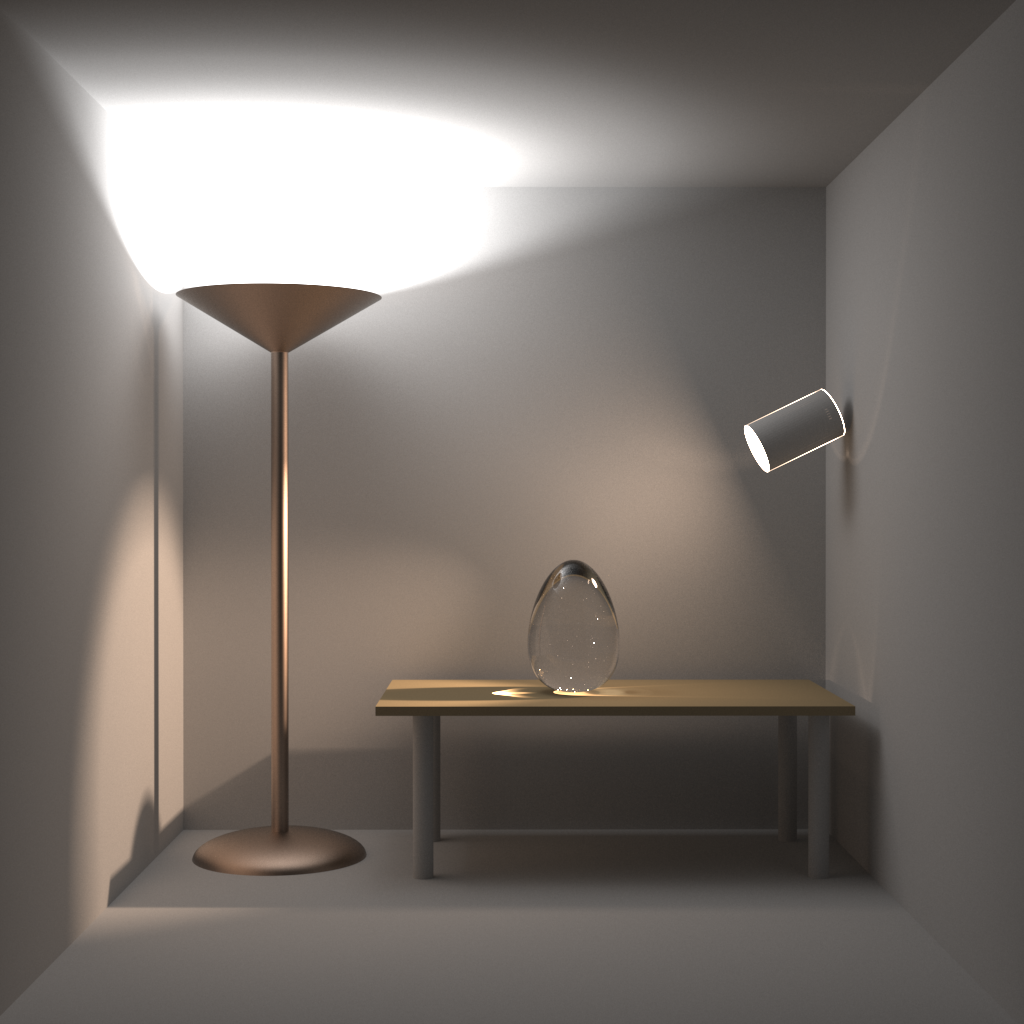
\includegraphics[width=2in]{figs/4_results/veach-bidir/1_from_mitsuba.png}
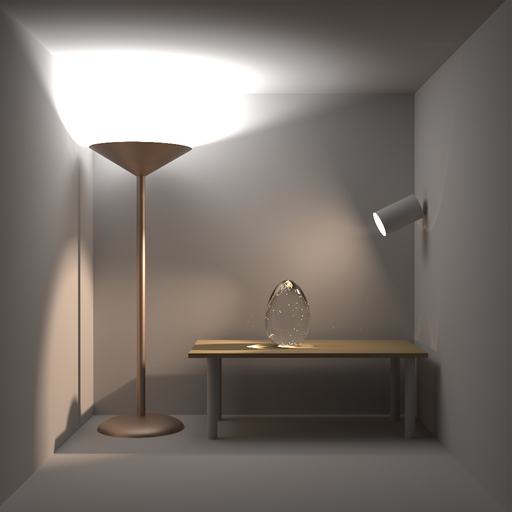
\includegraphics[width=2in]{figs/4_results/veach-bidir/2_to_pbrt.png}
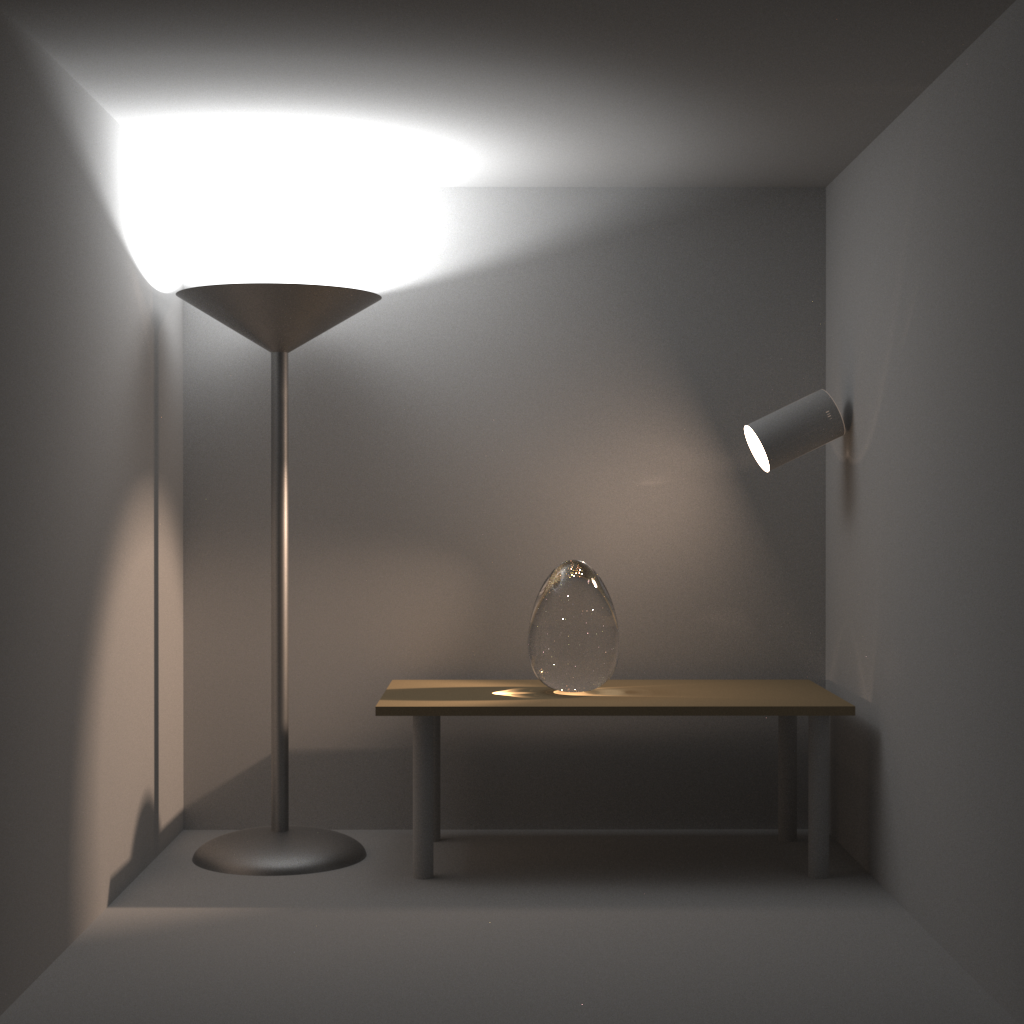
\includegraphics[width=2in]{figs/4_results/veach-bidir/3_to_lux.png}
\caption{Automatic conversion obtained with our system for \textit{Veach, Bidir Room}
scene originally modeled for Mitsuba. Rendering produced by Mitsuba (left).
Rendering produced by PBRT v3 (center) and LuxRender (right),
from converted scenes for the renderers}
\label{fig:veach-bidir}
\end{figure*}

%\begin{figure*}
%\centering
%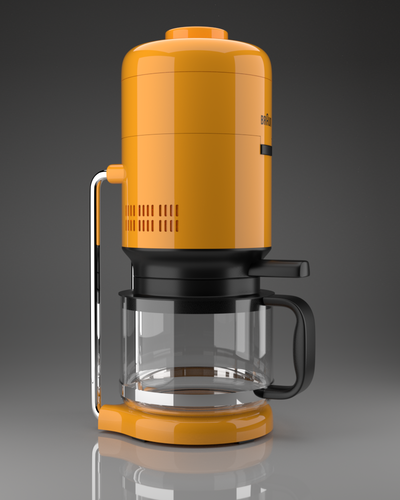
\includegraphics[width=2in]{figs/4_results/coffee/1_from_pbrt.png}
%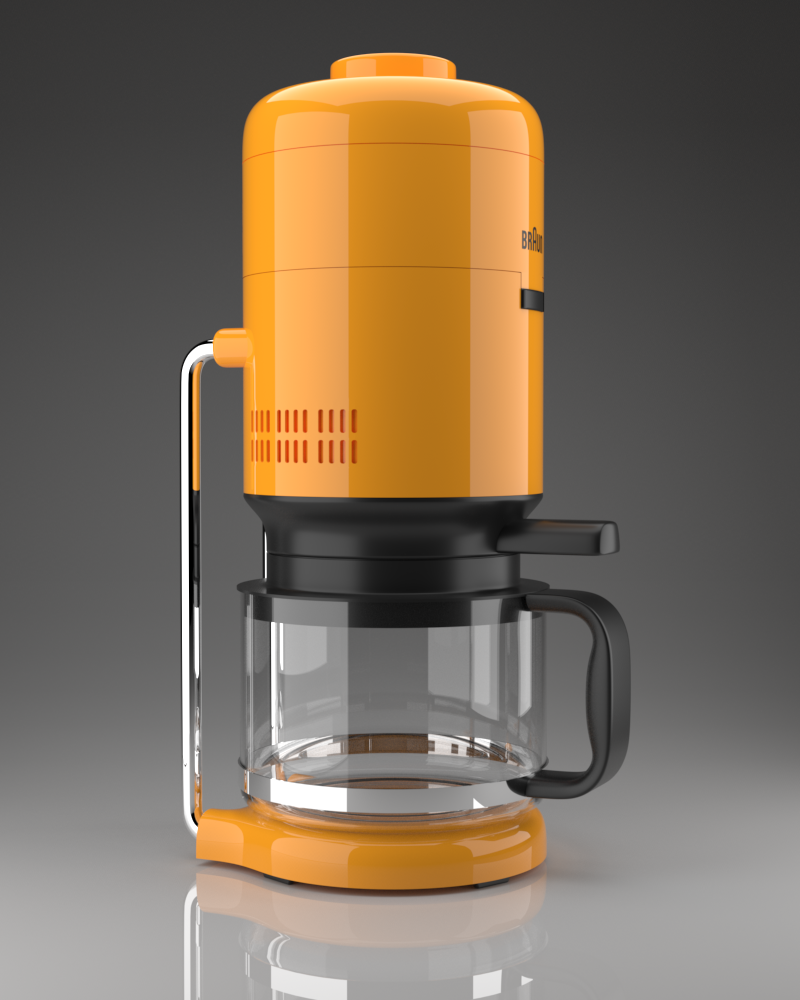
\includegraphics[width=2in]{figs/4_results/coffee/2_to_mitsuba.png}
%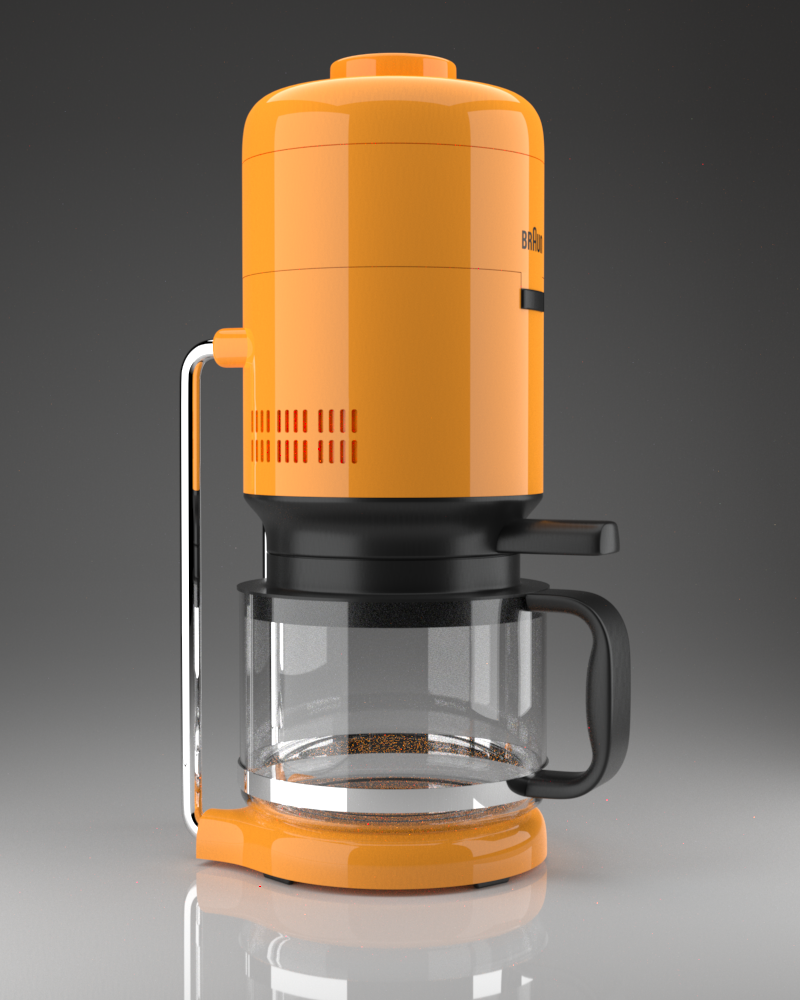
\includegraphics[width=2in]{figs/4_results/coffee/3_to_lux.png}
%\caption{Automatic conversion obtained with our system for \textit{Coffee Maker}
%scene originally modeled for PBRT v3. Rendering produced by PBRT v3 (left).
%Rendering produced by Mitsuba (center) and LuxRender (right),
%from converted scenes for the renderers}
%\label{fig:coffee}
%\end{figure*}




The results in Figure \ref{fig:staircase} differ a little in coloring from 
renderer to renderer due to the very nature of Monte Carlo Rendering - sampling 
can vary between scenes. The results obtained from our system were very similar 
to the original images.



\red{Obtaining the results in Figure \ref{fig:teapot} were particularly challenging}

\subsection{Limitations}
In order to minimize scope issues, we restricted the number of directives 
interpreted by our system. Generally speaking, directives present in only one 
renderer that had no correspondent in the other two renderers were not 
incorporated. That was the case, for instance, for Mitsuba-only materials like 
\textit{phong} or \textit{blendbsdf}. 

We chose not to interpret and convert hair or participating media (volumes, such 
as water or fog) for this PoC. We also did not convert the color for metal 
materials in LuxRender given the issues discussed in \ref{systemarch}.

We chose to limit the interpreted global emitters to the most commonly used 
ones: environment mapping, sun, sky, distant lighting, infinite. Therefore, spot 
and \red{point lights were not included in our PoC. [Why not?]}



